% Jaco Bezuidenhout
% 11013878

\begin{itemize}
	\item[] 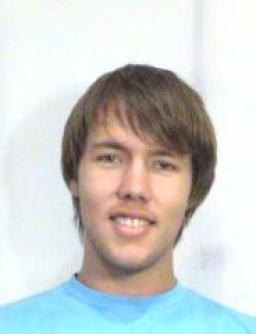
\includegraphics[scale=0.2]{Jaco}
	\item[] Jacobus Bezuidenhout
	\item Interests
	%Insert interests here
	\begin{itemize}
		\item Arduino
		\item Internet of Things (IoT)
		\item Electronics
		\item Remote Monitoring
		\item I like tracking things remotely and programming interaction with hardware.
	\end{itemize}
	\item Technical Skills
	%Insert technical skills here
	\begin{itemize}
		\item[] C, C++, Python, NodeJS, HTML(+js), Arduino and Microprocessors, PCB Design and Linux.
	\end{itemize}
	\item Past Experience
	%Insert past experience (relevant to the project) here
	\begin{itemize}
		\item[] I have created a few websites from scratch, and I'm currently hosting them on a VPS in Amsterdam, New York and London. My company is working on an animal tracking solution for the past 6 months. I also give training on the Intel Edison platform and electronics for Intel clients.
	\end{itemize}
	\item Non-technical Strengths
	%Insert non-technical strengths here
	\begin{itemize}
		\item[] I have good presentation and people skills, and I'm good with finding creative solutions.
	\end{itemize}
	\item Motivation for Project
	%Insert motivation here (why do you want to do the project)
	\begin{itemize}
		\item[] I have a soft spot for Rhinos and the conservation thereof. I also have a huge passion for remote monitoring and the IoT (Internet of Things) movement. This project and the technologies will not be so new to me because of the tracking solution I have developed for my company. My dream for this project is to know I have helped to keep the rhinos as part of our legacy.
	\end{itemize}
\end{itemize}